\graphicspath{{Baro_vort/code/plot_snap/figs/}}

We start with perhaps the most simple model of geophysical turbulence, barotropic vorticity model. We can write the model in vorticity form \parencite[\S 4.2.1]{Vallis_17}:
\begin{align}
    &\frac{\DD}{\DD t}\left( \{\text{Ro}^{-1}\}f+\zeta \right) = 0,\\
    &\zeta = \nabla^2\psi,\\
    &u = -\frac{\pe\psi}{\pe y}, v = \frac{\pe\psi}{\pe x}.
\end{align}
where
\begin{align}
    \text{Ro} = \frac{U}{fL}.
\end{align}

If $f$ is constant, it is the 2D incompressible Euler equation. We note that we do not use quasi-geostrophic to describe this model and reserve that name to the model with a finite deformation radius.

\section{Freely decaying simulation of 2D Euler}
We run freely decaying simulation with $f$ constant. We pick the initial energy containing scale of be around 1 and have a $15\times 15$ domain. We use $\nabla^8$ dissipation interpreted spectrally as $k^8+\ell^8$. 

Figure \ref{fig:2DEuler_zeta_t} shows the snap shots of vorticity and the streamfunction over the evolution of the simulation. We see a convincing inverse cascade and the formation of coherent vortices. Figure \ref{fig:2DEuler_energy} keep track of the kinetic energy and enstrophy. We see that, as expected, they experience a rapid initial decay. Afterwards, they are approximately conserved. Figure \ref{fig:2DEuler_spec} shows the evolution of the enstrophy spectra. The theoretical expectation is for them to have a $k^{-1}$ slope. We see that this is approximately true in early time. We also see that the hyper-dissipation is damping the small scale effectively.

\begin{figure}
    \centering
    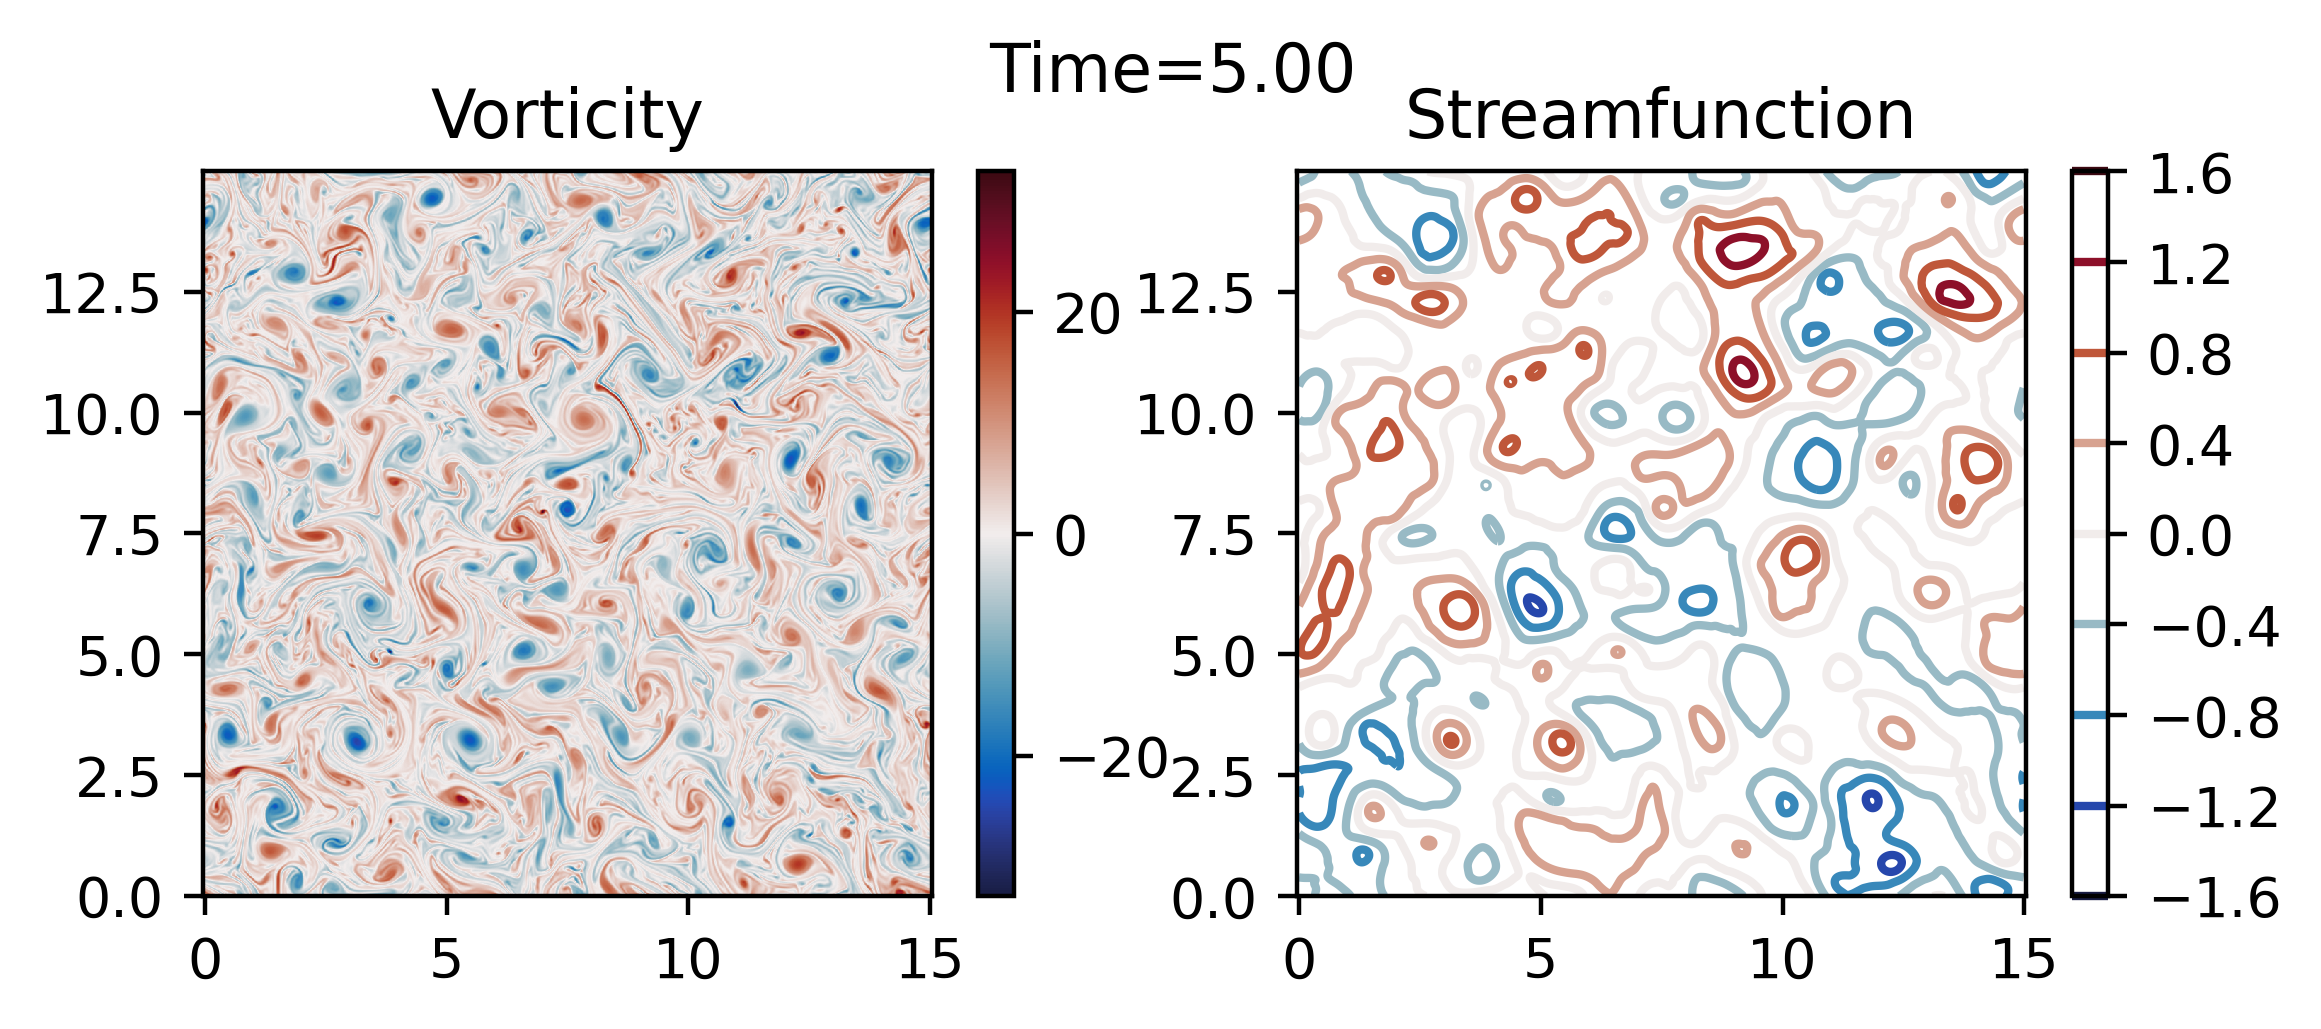
\includegraphics{2DEuler_zeta_t5d00}
    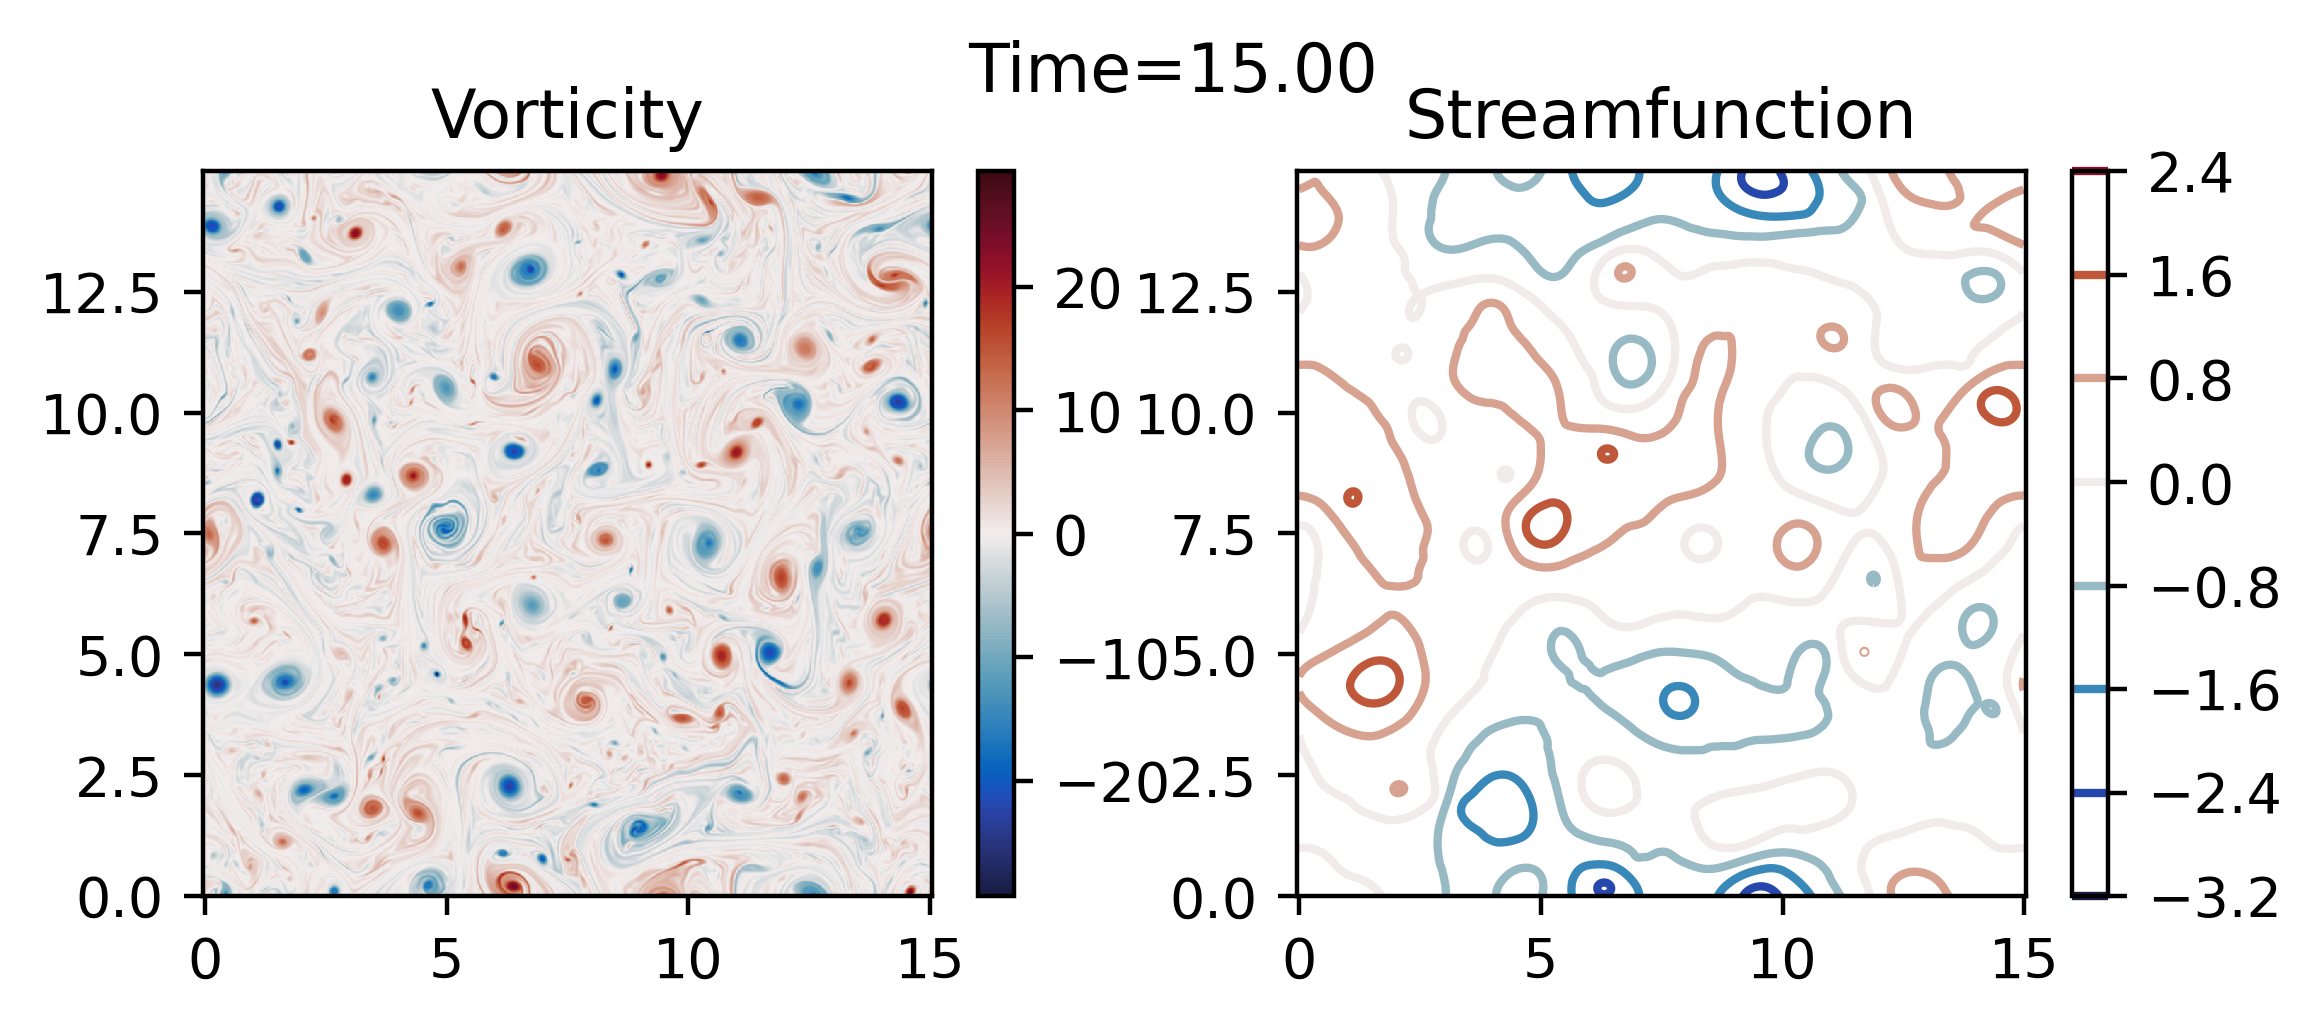
\includegraphics{2DEuler_zeta_t15d00}
    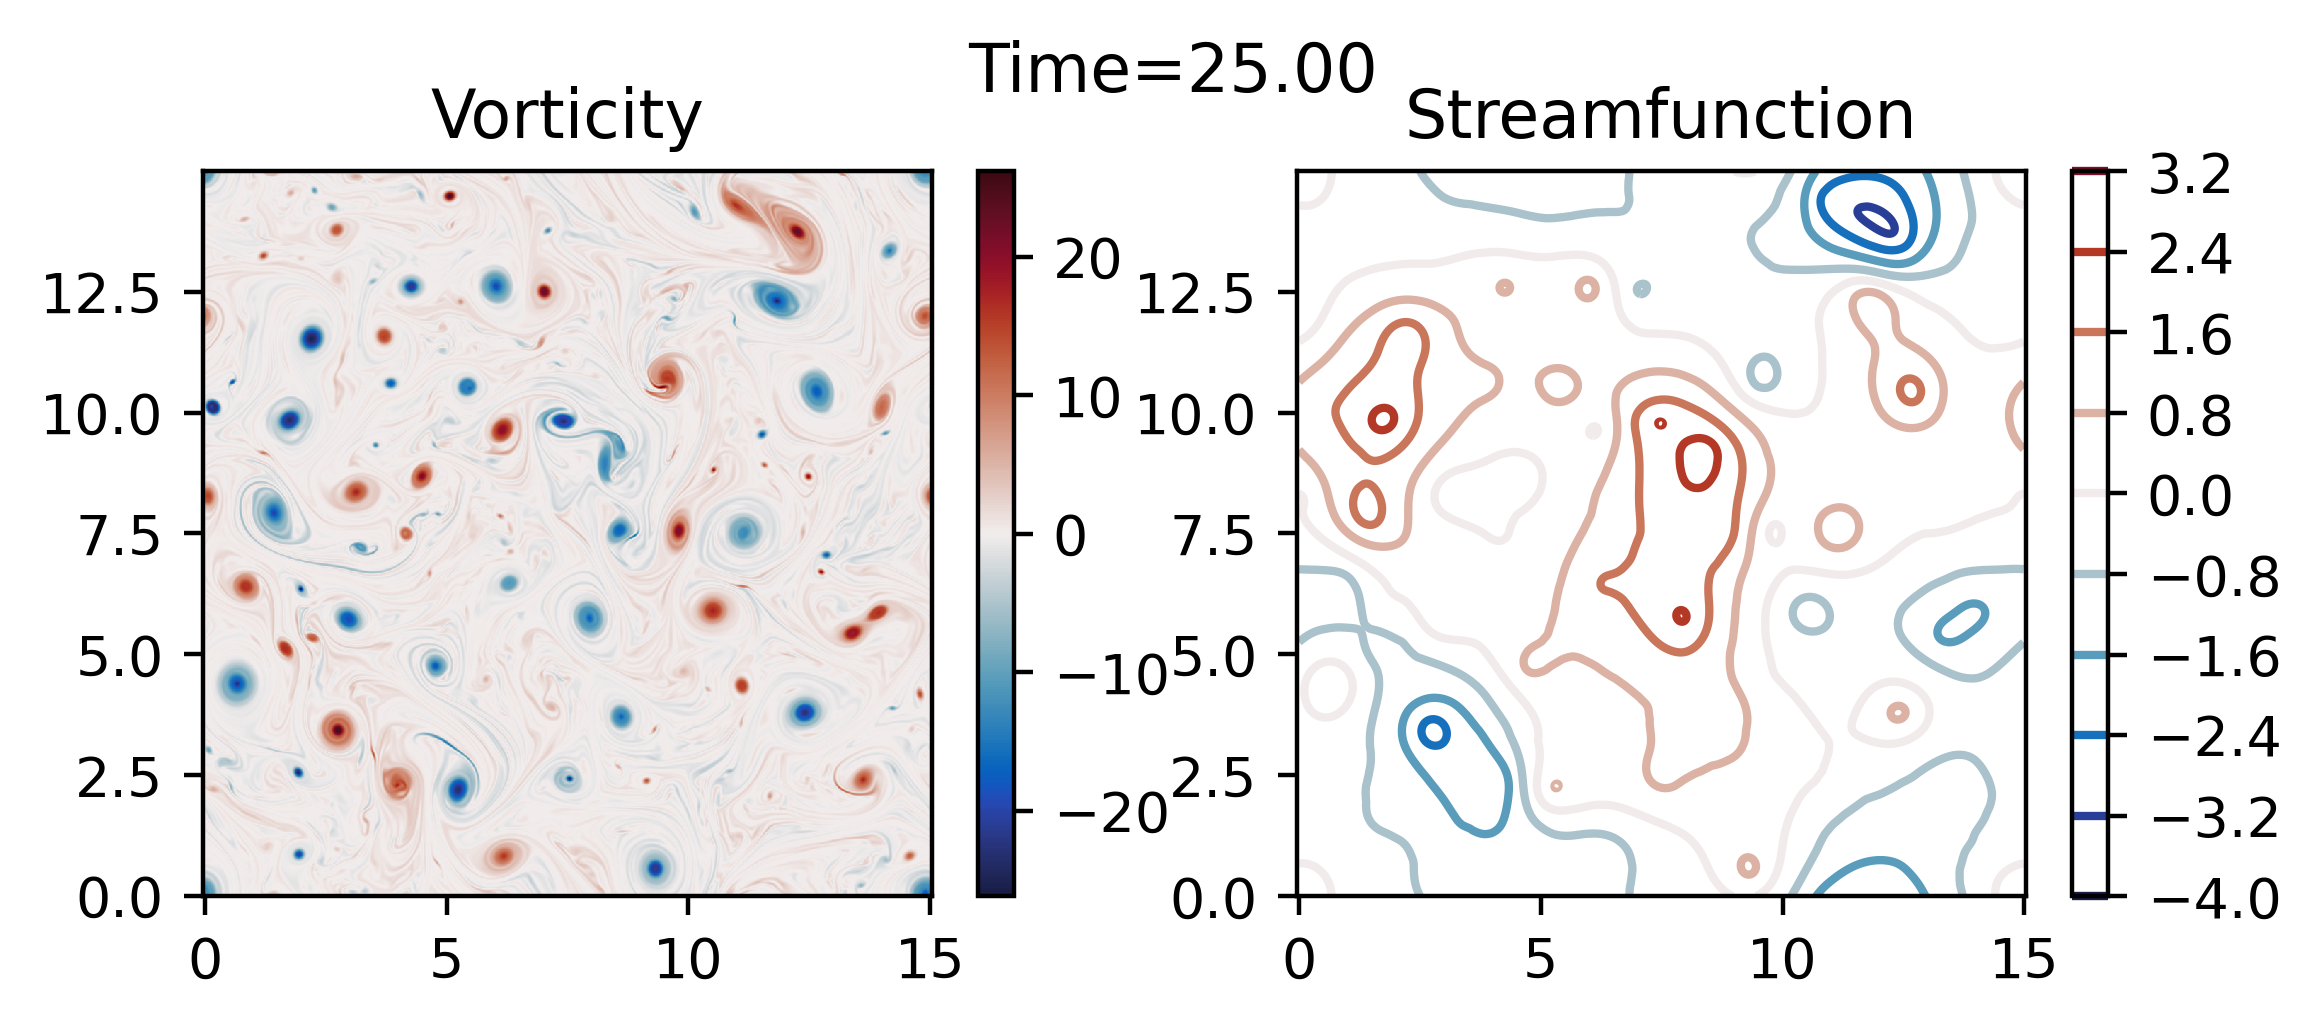
\includegraphics{2DEuler_zeta_t25d00}
    \caption{Snapshots of vorticity and streamfunction 2D Euler simulation overtime.}
    \label{fig:2DEuler_zeta_t}
\end{figure}

\begin{figure}
    \centering
    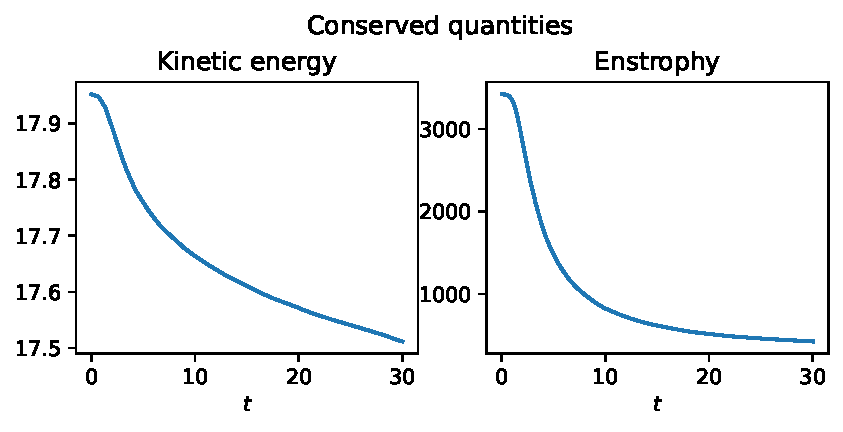
\includegraphics{2DEuler_energy}
    \caption{Time history of kinetic energy and enstrophy of 2D Euler simulation.}
    \label{fig:2DEuler_energy}
\end{figure}

\begin{figure}
    \centering
    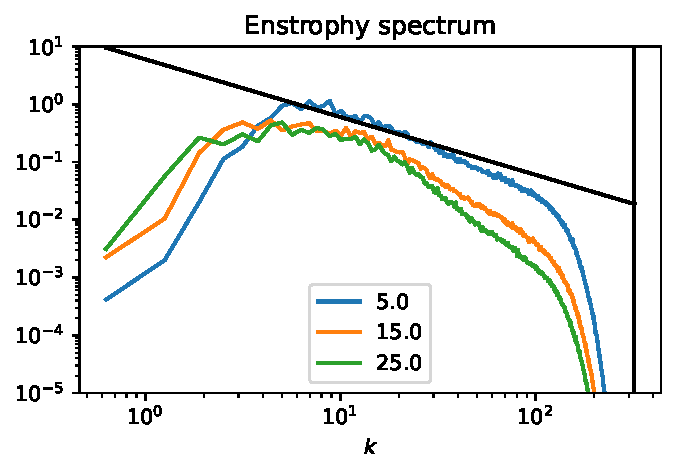
\includegraphics{2DEuler_spec}
    \caption{Time evolution of the enstrophy spectrum of 2D Euler simulation. Legends shows the time. The slanted black line is the $k^{-1}$ reference and the vertical black line is the maximally resolved wavenumber.}
    \label{fig:2DEuler_spec}
\end{figure}

% \section{Vortex crystal on a polar-cap}
% \cite[(2.2.10), p. 603]{Batchelor_53}

\section{Stochastically forced-dissipative simulation}


\section{Wind-forced gyres on a disk}
A particular application of the barotropic vorticity model is the models of wind-forced gyres \cite[\S 19.1.2.I]{Vallis_17}. Dedalus unable to use MPI parallelism when solving equations in a closed box. Therefore we choose to use a disk domain. In some loose sense, it captures the geometry of the Pacific. More importantly, this provides a chance to work with curvilinear domains in Dedalus.

We start with the full nonlinear barotropic vorticity equation on a $\beta$-plane \cite[(19.57)(19.59)]{Vallis_17}, \cite[\S 2]{IerleySheremet_95}:
\begin{align}
    \{R_\beta\}\left[\frac{\pe\zeta}{\pe t}+J(\psi,\zeta)\right]+\beta\frac{\pe\psi}{\pe x} = -\{\epsilon_s\}r\nabla^2\psi+\curl_z\ve\tau_T+\{\epsilon_M\}\nu\nabla^2\psi,
\end{align}
with
\begin{align}
    \psi(r=R) = 0 \qdt{and} \zeta(r=R) = 0.
\end{align}
We have the nondimensional numbers
\begin{align}
    R_\beta &= \frac{|\tau|}{\beta^2R^3};\\
    \epsilon_s &= \frac{r}{R\beta}\\
    \epsilon_M &= \frac{\nu}{\beta R^3}.
\end{align}
where $R$ is the diameter of the circle. 

We pick the 4 gyres wind forcing
\begin{align}
    \curl_z\ve\tau_T = -\sin(4\pi y/R) = -\sin(4\pi r\sin(\theta)/R).
\end{align}


\subsection{The linear Munk model}
We evolve the linear Munk model with $\epsilon_s=0.04$ (cf. \cite[Fig. 19.6]{Vallis_17}) in time till it reaches equilibrium. The model is
\begin{align}
    \beta\frac{\pe\psi}{\pe x}+\{\epsilon_s\}r\nabla^2\psi = \curl_z\ve\tau_T.
\end{align}
We determine that the model has converged by waiting till kinetic energy of the model has stopped changing (not shown) and by visual comparison of the output at different times. Figure \ref{fig:Gyre_stomlin_zetapsi} shows the equilibrated relative vorticity $\zeta$ and streamfunction $\psi$. We see that it looks similar to the Pacific gyres expect our model lack the equatorial dynamics while the real Pacific has the ACC instead of a subpolar gyre in the southern hemisphere.

\begin{figure}
    \centering
    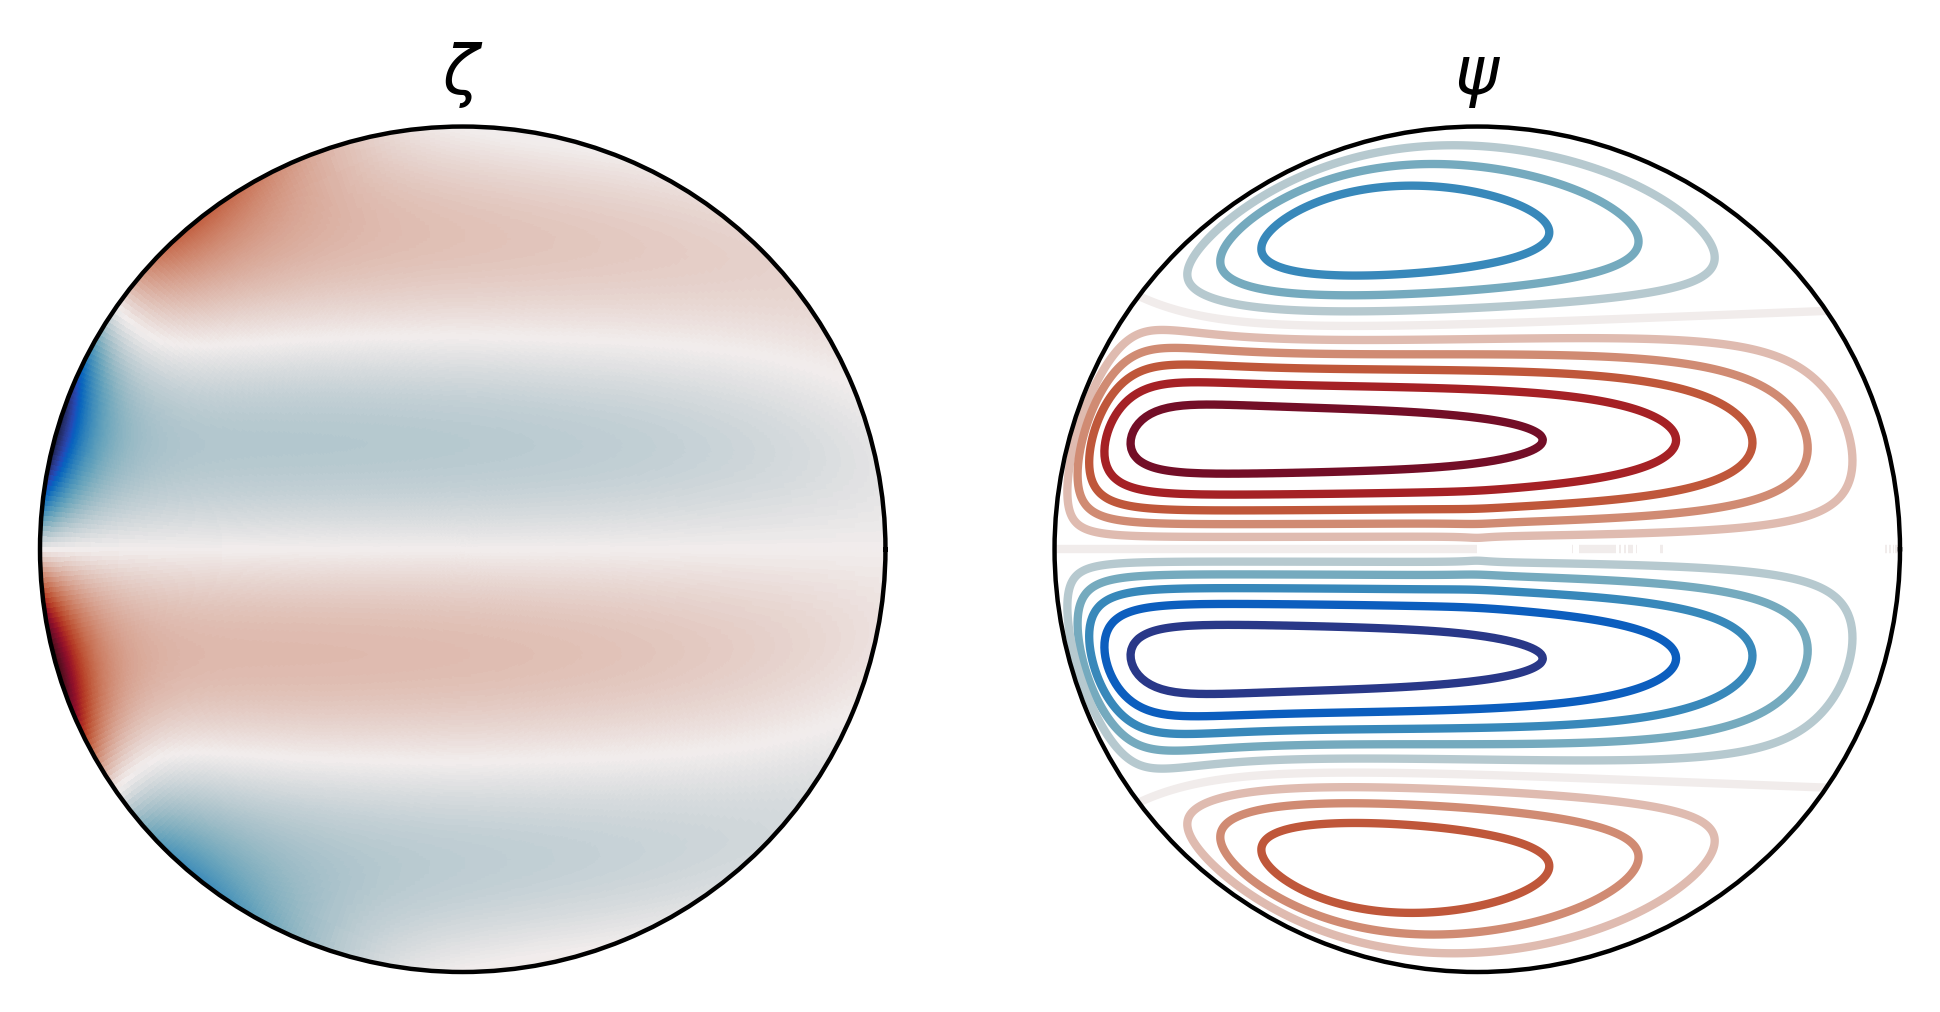
\includegraphics{Gyre_stomlin_zetapsi}
    \caption{Relative vorticity $\zeta$ and streamfunction $\psi$ of the equilibrated linear Munk model.}
    \label{fig:Gyre_stomlin_zetapsi}
\end{figure}

We note that this is a linear boundary value problem and Dedalus has a LBVP module. However, we have not been able to use it for this model because of our implementation of the $\zeta$ term using gradients. A proper solver using the LBVP feature is welcomed.

\subsection{The nonlinear Stommel model}
Now we solve the evolutionary nonlinear Stommel model
\begin{align}
    \{R_\beta\}\left[\frac{\pe\zeta}{\pe t}+J(\psi,\zeta)\right]+\beta\frac{\pe\psi}{\pe x} = \curl_z\ve\tau_T+\{\epsilon_M\}\nu\nabla^2\psi,
\end{align}
with $\epsilon_M = 0.06^3$ (cf. \cite{IerleySheremet_95}) and various value of $R_\beta$ for different nonlinear effects. In particular, the $S=0$ is the linear simulation with the $J(\psi,\zeta)$ term. All simulation has converged to equilibrium according to the the above definition. Figure \ref{fig:Gyre_munk_zetaall} shows the streamfunctions for simulation with different nonlinearities, titled by $S = \sqrt{R_\beta}$. This resembles the Munk (slip) case of \cite[Fig. 19.11]{Vallis_17}. We see that more stronger advection would push the circulation pattern towards the direction of the flow, eventually separating the subtropical gyres into two smaller ones. We also see the more nonlinear simulation has less pronounced western boundary currents. This is consistent with the results of \cite[Fig. 19.11]{Vallis_17} and \cite[Figure 2]{IerleySheremet_95}.

It is known that the nonlinear Munk model has multiple stable equilibriums in certain parameter regimes \parencite{CessiIerley_95, IerleySheremet_95}. Our time evolution method could be adapted to change the parameters slowly (via restarting) to find the equilibriums. We do not pursue that direction here any further.

\begin{figure}
    \centering
    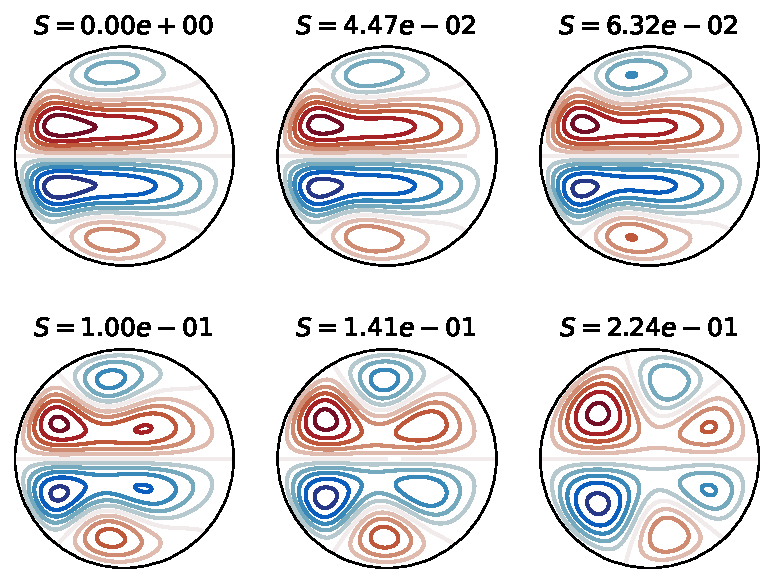
\includegraphics{Gyre_munk_zetaall}
    \caption{Streamfunctiona $\psi$ of the equilibrated nonlinear Munk model titled by $S = \sqrt{R_\beta}$}
    \label{fig:Gyre_munk_zetaall}
\end{figure}